\section{Dataset }
Our dataset consists of 105841 .wav files in 41 folders in random order. 

\subsection{Source }
Pytorch Speechcommand dataset Link: \\
(\url {https://pytorch.org/audio/stable/datasets.html#speechcommands})
\subsection{Data Sample  }
The data set samples are elaborated as follows:
    \begin{figure}[ht]
            \centering
            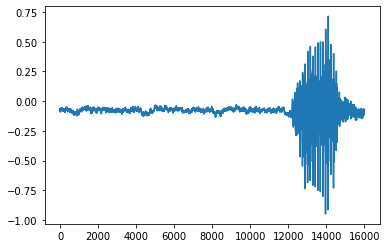
\includegraphics[scale=1]{images/figure4.png}
            \caption{Block diagram of Mel spectrogram of an audio signal.}
            \label{fig: Block diagram of Mel spectrogram of an audio signal}
            \end{figure}
We can comprehend two things after looking at the waveform and the label. Since the labels are text, we must first translate them into class numbers. Second, we confirm that each data sample, or 1x16000, is the same length.            
\section{Data Preprocessing }
\subsection{Normalization}
We will be talking 1x16000 waveforms.  So, after analyze there are some files that are not fulfill our requirements. Then we drop approximately 10,000 samples and we have 95394 data samples after normalizations.